\documentclass[11pt,letterpaper]{article}
\usepackage[utf8]{inputenc}
\usepackage[T1]{fontenc}
\usepackage[spanish,es-tabla]{babel}
\usepackage{amsmath,amssymb,amsfonts}
\usepackage{graphicx}
\usepackage{booktabs}
\usepackage{geometry}
\usepackage{float}
\usepackage{caption}
\usepackage{subcaption}
\usepackage{hyperref}
\usepackage{array}

\geometry{left=2.5cm, right=2.5cm, top=2.5cm, bottom=2.5cm}
\decimalpoint

\hypersetup{
    colorlinks=true,
    linkcolor=blue,
    urlcolor=blue,
    citecolor=blue
}


\title{\textbf{Tarea 3: Técnicas de Selección}}
\author{\textbf{Carlos Antonio Carreño Castaños}}
\date{\today}

\begin{document}

\maketitle


\section{Resultados}

Primero se generó una población inicial de $N = 20$ individuos ordenados de forma ascendente según su valor de adaptación (\textit{fitness}), el cual osciló entre $121$ (Individuo \#1) y $988$ (Individuo \#20), obteniendo una suma total de adaptación de $11\,909$ y un promedio poblacional inicial de $\bar{f} = 595.45$. En la Tabla \ref{tab:conteo_seleccion} se presentan los conteos de copias asignadas por cada técnica frente al valor esperado teórico $e_i = (f_i / \bar{f})$.

\begin{table}[H]
\centering
\caption{Conteo de copias seleccionadas por individuo para cada técnica de selección ($N = 20$).}
\label{tab:conteo_seleccion}
\resizebox{\textwidth}{!}{%
\begin{tabular}{@{}ccccccccccc@{}}
\toprule
\textbf{Ind.} & \textbf{Fitness ($f_i$)} & \textbf{Val. Esp. ($e_i$)} & \textbf{Ruleta} & \textbf{Sob. CR} & \textbf{Sob. SR} & \textbf{SUS} & \textbf{M. Det.} & \textbf{T. Det. ($k=3$)} & \textbf{T. Prob. ($p=0.75$)} & \textbf{Uniforme} \\ \midrule
\#1  & 121 & 0.203 & 0 & 0 & 0 & 0 & 0 & 0 & 1 & 2 \\
\#2  & 274 & 0.460 & 0 & 0 & 0 & 1 & 1 & 0 & 2 & 1 \\
\#3  & 339 & 0.569 & 0 & 1 & 1 & 0 & 1 & 0 & 0 & 1 \\
\#4  & 366 & 0.615 & 1 & 0 & 1 & 1 & 1 & 0 & 3 & 1 \\
\#5  & 444 & 0.746 & 0 & 0 & 1 & 1 & 1 & 0 & 0 & 0 \\
\#6  & 447 & 0.751 & 2 & 1 & 0 & 1 & 1 & 0 & 0 & 0 \\
\#7  & 464 & 0.779 & 0 & 2 & 1 & 0 & 1 & 0 & 1 & 0 \\
\#8  & 550 & 0.924 & 2 & 3 & 1 & 1 & 1 & 0 & 0 & 1 \\
\#9  & 571 & 0.959 & 1 & 1 & 1 & 1 & 1 & 1 & 0 & 0 \\
\#10 & 606 & 1.018 & 0 & 1 & 1 & 1 & 1 & 0 & 1 & 3 \\
\#11 & 675 & 1.134 & 0 & 1 & 1 & 1 & 1 & 0 & 0 & 3 \\
\#12 & 693 & 1.164 & 1 & 1 & 1 & 2 & 1 & 1 & 1 & 0 \\
\#13 & 698 & 1.172 & 1 & 1 & 1 & 1 & 1 & 1 & 2 & 1 \\
\#14 & 708 & 1.189 & 2 & 1 & 1 & 1 & 1 & 2 & 0 & 1 \\
\#15 & 767 & 1.288 & 2 & 1 & 1 & 1 & 1 & 3 & 1 & 2 \\
\#16 & 770 & 1.293 & 1 & 1 & 2 & 1 & 1 & 7 & 1 & 1 \\
\#17 & 772 & 1.296 & 0 & 1 & 2 & 2 & 1 & 1 & 1 & 0 \\
\#18 & 821 & 1.379 & 1 & 1 & 1 & 1 & 1 & 0 & 3 & 2 \\
\#19 & 835 & 1.402 & 4 & 1 & 1 & 2 & 1 & 2 & 0 & 0 \\
\#20 & 988 & 1.659 & 2 & 2 & 2 & 1 & 2 & 2 & 3 & 1 \\ \midrule
\textbf{Total} & \textbf{11909} & \textbf{20.000} & \textbf{20} & \textbf{20} & \textbf{20} & \textbf{20} & \textbf{20} & \textbf{20} & \textbf{20} & \textbf{20} \\ \bottomrule
\end{tabular}%
}
\end{table}

En la Tabla \ref{tab:conteo_seleccion}, se observa cómo responde cada método ante la distribución de la población:
\begin{itemize}
    \item \textbf{Efecto del azar en la Ruleta vs. Métodos de Baja Varianza:} En la \textbf{Ruleta}, el giro independiente en cada selección provocó que individuos por encima del promedio como el \#10 ($f_{10} = 606$), el \#11 ($f_{11} = 675$) y el \#17 ($f_{17} = 772$, con $e_{17} = 1.296$) quedaran con $0$ copias, mientras que el individuo \#19 ($e_{19} = 1.402$) acumuló $4$ copias. En cambio, la \textbf{Selección Universal Estocástica (SUS)} y los métodos de \textbf{Sobrante Estocástico} aseguraron como mínimo la parte entera $\lfloor e_i \rfloor = 1$ para todos los individuos del \#10 al \#20, evitando que soluciones aptas fueran descartadas por azar.
    \item \textbf{Asignación de residuos en Sobrante y Muestreo Determinístico:} Debido a que los once individuos superiores (\#10 al \#20) tuvieron una parte entera de $\lfloor e_i \rfloor = 1$, quedaron $9$ cupos por repartir mediante las partes fraccionarias ($e_i - \lfloor e_i \rfloor$). En el \textbf{Sobrante con Reemplazo}, el individuo \#8 ($e_8 = 0.924$) poseía una parte decimal muy alta y resultó elegido $3$ veces en la ruleta de residuos, mientras que en el \textbf{Sobrante sin Reemplazo} ningún individuo superó las $2$ copias. Asimismo, en el \textbf{Muestreo Determinístico}, dado que los individuos del \#2 al \#9 tenían partes decimales ($0.460$ a $0.959$) mayores que los residuos de los individuos \#10 al \#19 ($0.018$ a $0.402$), los $9$ cupos restantes se asignaron exactamente a los individuos \#2 al \#9 y al \#20 ($0.659$), dejando una distribución uniforme de $1$ copia entre el \#2 y el \#19 y $2$ copias en el \#20.
    \item \textbf{Comportamiento de los Torneos:} El \textbf{Torneo Determinístico ($k=3$)} descartó por completo a los primeros ocho individuos (\#1 al \#8 con $0$ copias) y concentró $7$ selecciones en el individuo \#16 ($f_{16} = 770$). Por el contrario, el \textbf{Torneo Probabilístico ($k=2, p=0.75$)}, al otorgar un $25\%$ de probabilidad de victoria al competidor menos apto, permitió que individuos bajos como el \#1, \#2 y \#4 conservaran copias en la siguiente generación.
\end{itemize}

Posteriormente, se calculó el fitness promedio ponderado de los padres elegidos y el número máximo de repeticiones de un mismo individuo para medir el favorecimiento de los mejores individuos y la conservación de diversidad, cuyos resultados se muestran en la Tabla \ref{tab:presion_selectiva}.

\begin{table}[H]
\centering
\caption{Resumen comparativo de la selectividad de cada técnica.}
\label{tab:presion_selectiva}
\begin{tabular}{@{}l >{\centering\arraybackslash}p{3.8cm} >{\centering\arraybackslash}p{3.6cm}@{}}
\toprule
\textbf{Técnica de Selección} & \textbf{Fitness Promedio de Padres} & \textbf{Máximo de Copias de 1 Individuo} \\ \midrule
Población Inicial (Referencia sin selección)    & 595.45 & 1 \\ \midrule
1. Ruleta (SP)                                  & 708.95 & 4 \\
2.1 Sobrante Estocástico con Reemplazo (SP)     & 662.80 & 3 \\
2.2 Sobrante Estocástico sin Reemplazo (SP)     & 679.85 & 2 \\
3. Universal Estocástica -- SUS (SP)            & 664.25 & 2 \\
4. Muestreo Determinístico (SP)                 & 638.80 & 2 \\
5.1 Torneo Determinístico ($k=3$) (ST)          & 774.35 & 7 \\
5.2 Torneo Probabilístico ($k=2, p=0.75$) (ST)  & 633.10 & 3 \\
6. Selección Uniforme (SU)                      & 597.70 & 3 \\ \bottomrule
\end{tabular}
\end{table}

\begin{figure}[H]
    \centering
    \IfFileExists{img_prueba.png}{%
        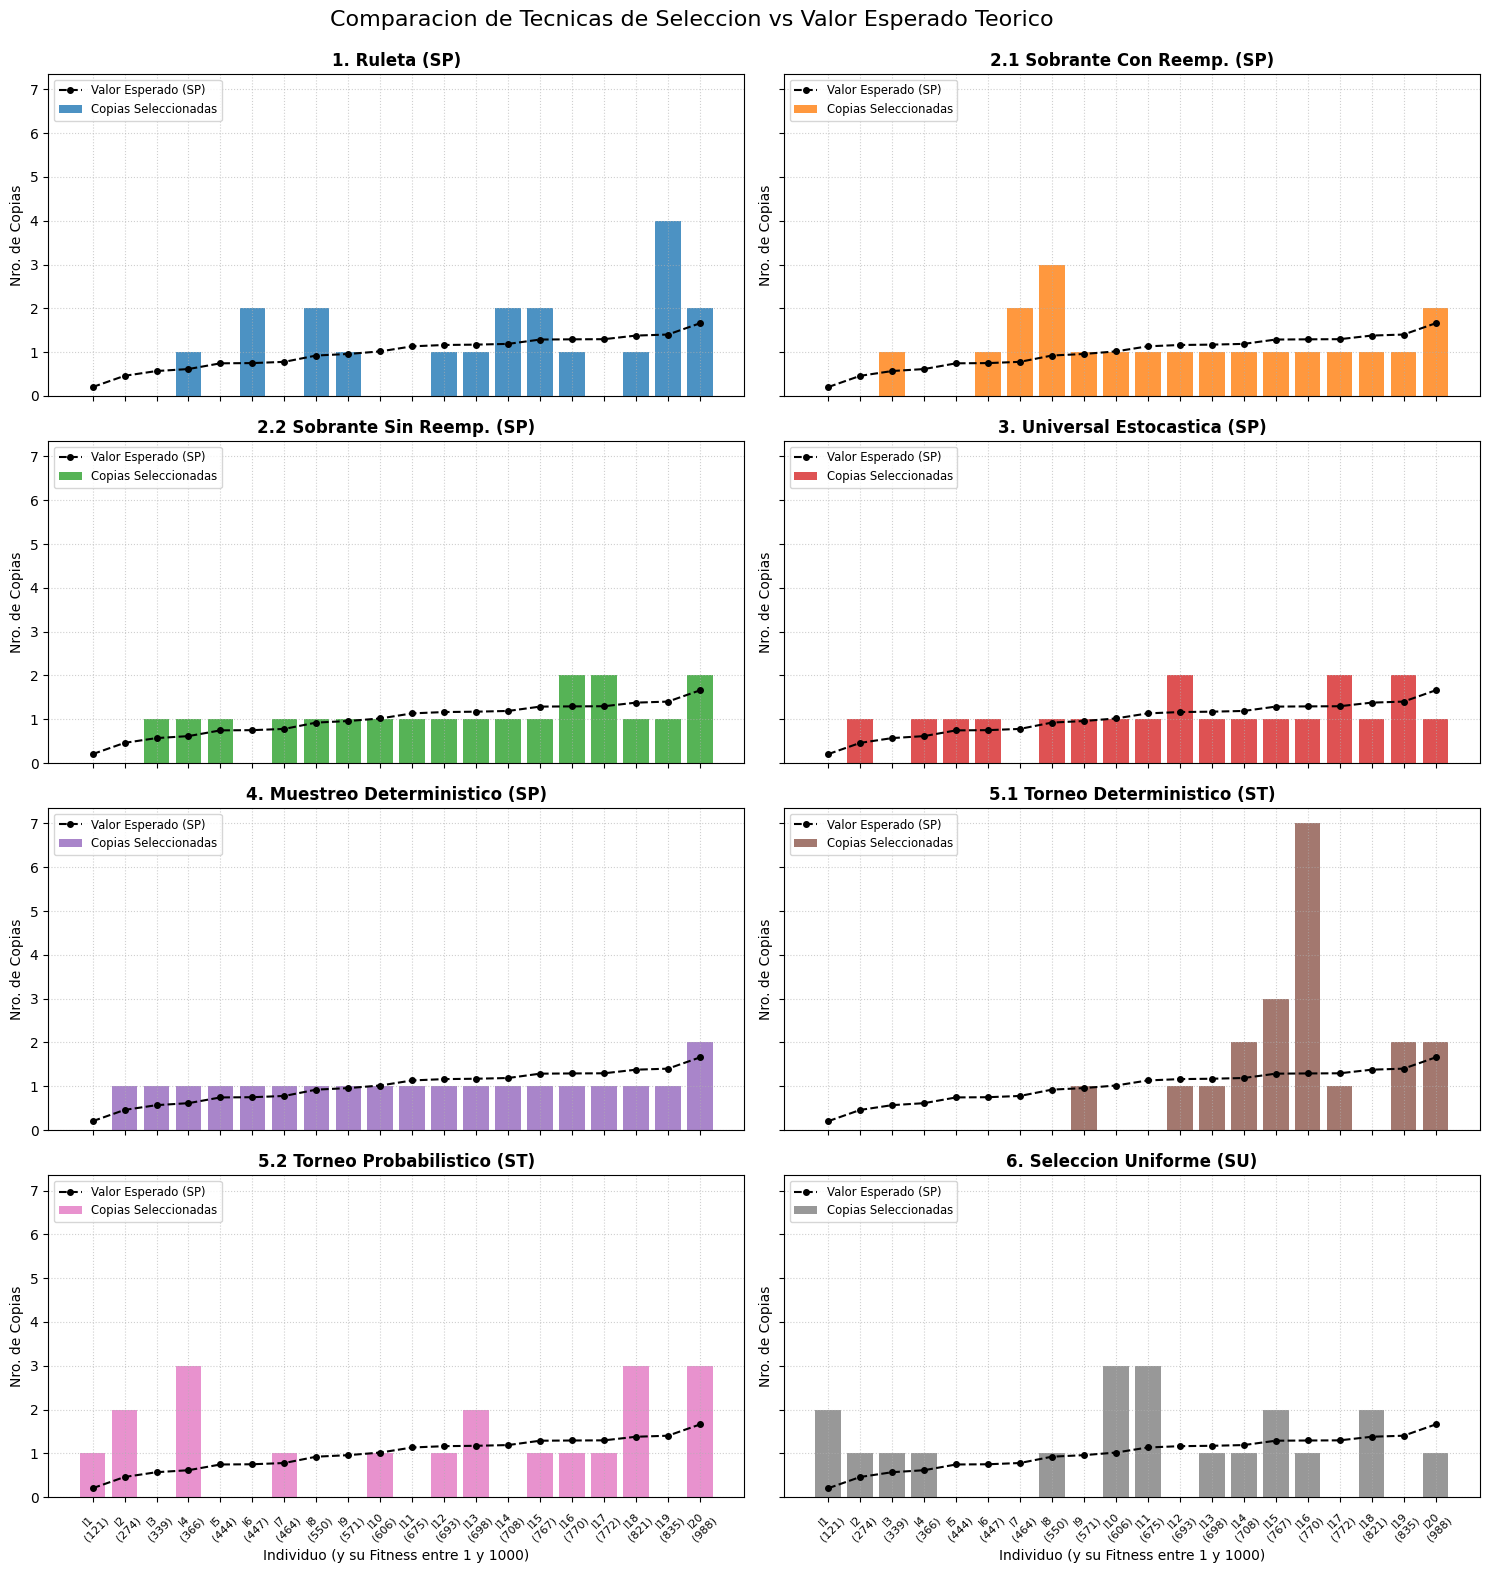
\includegraphics[width=0.95\textwidth]{img_prueba.png}%
    }{%
        \fbox{\parbox{0.9\textwidth}{\centering \vspace{1.2cm} \textit{[Colocar imagen como \texttt{output\_20\_1.png}: Panel comparativo de las 8 técnicas de selección vs. Valor Esperado Teórico]} \vspace{1.2cm}}}%
    }
    \caption{Comparación gráfica del número de copias seleccionadas por individuo frente a la curva de valor esperado teórico ($e_i$).}
    \label{fig:panel_seleccion}
\end{figure}

Como se aprecia en la Tabla \ref{tab:presion_selectiva} y en las gráficas de la Figura \ref{fig:panel_seleccion}, el \textbf{Torneo Determinístico ($k=3$)} produjo el mayor favorecimiento de los mejores individuos de todas las pruebas, elevando el fitness promedio de la población desde $595.45$ hasta $774.35$; sin embargo, al asignar $7$ copias a un mismo individuo, introduce el riesgo de perder diversidad genética prematuramente. Por su parte, las técnicas de \textbf{Sobrante sin Reemplazo ($679.85$)} y \textbf{Universal Estocástica ($664.25$)} lograron incrementar de manera efectiva la aptitud media de los padres manteniendo un máximo de apenas $2$ copias por individuo. Finalmente, la \textbf{Selección Uniforme} arrojó un promedio de $597.70$, un valor idéntico a la media inicial de $595.45$, comprobando que al seleccionar padres con probabilidad constante no existe empuje evolutivo hacia mejores soluciones.

% ==============================================================================
%\section{Conclusiones}
% ==============================================================================
%\begin{enumerate}
%    \item La \textbf{Selección Universal Estocástica (SUS)} y el \textbf{Sobrante Estocástico sin Reemplazo} demostraron el mejor equilibrio entre favorecimiento de los mejores individuos y preservación de diversidad dentro de los métodos proporcionales, logrando seguir de cerca la curva de valor esperado $e_i$ con un tope máximo de $2$ copias por individuo y sin las omisiones por azar observadas en la Ruleta.
%    \item El \textbf{Muestreo Determinístico} elimina por completo la varianza del muestreo al asignar primero las partes enteras y luego ordenar los residuos decimales; no obstante, cuando la población presenta valores esperados levemente superiores a la unidad ($1.0 < e_i < 1.5$), las partes fraccionarias más altas se concentran en los individuos de adaptación media-baja ($e_i \approx 0.7 - 0.9$), moderando su favorecimiento de los mejores individuos ($638.80$).
%    \item La \textbf{Selección por Torneo} permite controlar directamente la intensidad evolutiva sin necesidad de calcular sumatorias globales de fitness: el esquema determinístico ($k=3$) acelera fuertemente la convergencia hacia los individuos más aptos ($774.35$), mientras que el esquema probabilístico ($p=0.75$) suaviza dicho favorecimiento de los mejores individuos ($633.10$) para mantener variabilidad genética.
%    \item La \textbf{Selección Uniforme} mantuvo el fitness promedio de los padres ($597.70$) casi inalterado respecto a la población original ($595.45$), confirmando que el favorecimiento de los mejores individuos guiado por la función de adaptación es indispensable para que el algoritmo genético evolucione.
%\end{enumerate}

\end{document}